% THIS IS SIGPROC-SP.TEX - VERSION 3.1
% WORKS WITH V3.2SP OF ACM_PROC_ARTICLE-SP.CLS
% APRIL 2009
%
% It is an example file showing how to use the 'acm_proc_article-sp.cls' V3.2SP
% LaTeX2e document class file for Conference Proceedings submissions.
% ----------------------------------------------------------------------------------------------------------------
% This .tex file (and associated .cls V3.SP) *DOES NOT* produce:
%       1) The Permission Statement
%       2) The Conference (location) Info information
%       3) The Copyright Line with ACM data
%       4) Page numbering
% ---------------------------------------------------------------------------------------------------------------
% It is an example which *does* use the .bib file (from which the .bbl file
% is produced).
% REMEMBER HOWEVER: After having produced the .bbl file,
% and prior to final submission,
% you need to 'insert'  your .bbl file into your source .tex file so as to provide
% ONE 'self-contained' source file.

\documentclass{acm_proc_article-sp}

\usepackage{amsmath}
\usepackage{mathptmx}
\usepackage{times}
\usepackage{verbatim}
\usepackage{graphicx,subfigure}
\usepackage{color}
\usepackage[boxed]{algorithm2e}
\DontPrintSemicolon
\SetArgSty{}

\newcommand{\TODO}[1]{\textcolor{red}{(#1)}}

\newcommand{\reals}{{\textit I\!\hspace{-0.025em} R}}
\newtheorem{theorem}{Theorem}[section]
\newtheorem{lemma}[theorem]{Lemma}
\newtheorem{obssoervation}[theorem]{Observation}
\newtheorem{observationdefinition}[theorem]{Observation}
\newtheorem{corollary}[theorem]{Corollary}
\newtheorem{definition}[theorem]{Definition}
\newtheorem{problem}[theorem]{Problem}
\newtheorem{property}[theorem]{Property}

\newcommand{\Frechet}[0]{Fr\'{e}chet}
\newcommand{\TMATCH}{\textsc{TMATCH}}

\begin{document}

\title{Trajectory Mosaicing}

\numberofauthors{2} %  in this sample file, there are a *total*
\author{
\alignauthor
E.~Packer\\
       \affaddr{IBM Research - Haifa}\\
       \affaddr{University of Haifa Campus}\\
       \affaddr{Haifa, Israel 3498825}\\
\alignauthor
S.~Pupyrev, A.~Efrat, S.~Kobourov \\
       \affaddr{Department of Computer Science}\\
       \affaddr{University of Arizona}\\
\affaddr{Tucson, AZ, USA}
}

\maketitle
\begin{abstract}
The ubiquitous presence of location-based devices and sensors has made it easier to collect data on the trajectories of people, animals, vehicles, and objects. The benefits of collecting this data are clear, whether for traffic analysis, social analytics, business optimization, or safety measures. Unfortunately, much of the data on these trajectories is incomplete or unreliable, and cannot be used �as is� for further analytics. We introduce new methods to combine and process trajectory data. In the core of this work we present a system to analyze ant trajectories annotated manually. Our work reviews the difficulties and challenges that arise in this scenario and presents efficient solutions 
with which we obtained satisfactory results. These solutions which relate
to trajectories and deal with clustering and matching are generic enough
to be used in many systems that require trajectory analysis. In particular, systems that process incomplete data or suffer from reasonable noise could benefit from our solutions. We implemented the methods and present experiments with real-world data. TODO{ It would be good to say something here about the results to provide credibility and give people a reason to read the paper]}

\end{abstract}

\category{H.4}{Information Systems Applications}{Miscellaneous}
\terms{Algorithms}
\keywords{Trajectories, Matching}


%%%%%%%%%%%%%%%%%%%%%%%%%%%%%%%%%%%%%%%%%%%%%%%%%%%%%%%%%%%%%%%%%%%%%%%%%%%
%%%%%%%%%%%%%%%%%%%%%%%%%%%%%%%%%%%%%%%%%%%%%%%%%%%%%%%%%%%%%%%%%%%%%%%%%%%
%%%%%%%%%%%%%%%%%%%%%%%%%%%%%%%%%%%%%%%%%%%%%%%%%%%%%%%%%%%%%%%%%%%%%%%%%%%
%%%%%%%%%%%%%%%%%%%%%%%%%%%%%%%%%%%%%%%%%%%%%%%%%%%%%%%%%%%%%%%%%%%%%%%%%%%
\section{Introduction}
[Explain the idea of Mosaicing.]
Due to the availability of location enabled devices, data with spatial attributes has become more and more widespread, increasing the demand for analytical tools.
Numerous technologies are available to provide location data, including GPS, WiFi, cellolar and cameras. Moreover, many applications that make use of this location data have been developed and are available for mobile phones, navigation systems, and more.

\TODO{Clearly state the problem here and the importance of your results}

{\it Trajectories} are arguably the most interesting pieces of information created by location services.
\TODO{Move the details to a subsequent section} Let a {\em trajectory} be defined as a polyline in $\reals^2$, represented by
a sequence $p_1, \dots, p_m$ of $m$ points. In addition to the spatial
coordinates, temporal information might also be available.
Specifically, each point $p_i$ is associated with a normalized timestamp $0 \le t_i \le 1$ and we assume that the 
trajectory is monotone in time: for each $1 < i < j < T$, it holds $t_1 = 0 < t_i < t_j < t_T = 1$. Hence, a 
trajectory can be viewed as a monotone (with respect to time) polyline in the
$\reals^3$ domain with the coordinates $x$, $y$ and $t$.
In our settings, we usually parameterize (or normalize) the timestamp along the
interval $[0, 1]$.
%A \emph{distance} between a pair of trajectories is defined as the maximum
% distance between the corresponding polylines at any timestamp. Let $u,v$ be a pair of trajectories, and $D(u(t), v(t))$ denote the distance
%between $u$ and $v$ at the timestamp $t$. Then the distance between $u$ and $v$
% is $$D(u, v) = \max_{t \in [0,1]} D(u(t), v(t)).$$

Many applications use the trajectory data as historical resources, including statistics about outdoor activities, 
common route analysis, and traffic congestion analysis. Other applications use the data on-the-fly for current route 
statistics, the analysis of  current relationships with other trajectories, and more.
Trajectories for ships, airplanes, animals, and even people are constantly being collected
and used in academic and industrial research.

The availability of trajectory data offer unique opportunities to gain insight. For example, analyzing the complicated relationships 
among trajectories can help alleviate traffic congestion and thus save time and money, while decreasing pollution.
%Another related problem is route optimization. Given the source and destination, it could be valuable to decide both the route taken by the vehicles as well as scheduling its route stations. Last but not least, today's available communication allows real time transportation on demand (taxis, merchandize shipping, emergency vehicles, etc.). Given services and requests, it would be important to optimize the routes and their scheduling in real-time.
Trajectory data can also be used to examine human mobility and social patterns~\cite{isaacman10}. Such understanding can,
in turn, help advance solutions to large-scale societal problems in fields as varied as telecommunications, ecology, 
epidemiology, and urban planning. For example, knowing how large populations of people move about can help determine their carbon footprint and subsequently guide policies intended to reduce that footprint.

%Trajectory data, together with growing demand to analyze such data, pose many
% challenges. For example, real-time travel route calculation is a difficult problem. Another challenge is related to location and time inaccuracies associated with input trajectories. Inevitably, location signals are noisy, contain outliers, and have unexpected behavior.
%Removing noise and fixing trajectories may be of great value to achieve the correct conclusions.

Over the years, many problems that relate to trajectories have been proposed and
solved. Four common problems relate to: measuring the distances
between pairs of trajectories, matching sets of trajectories, clustering
trajectories, and computing common routes. These problems have been
extensively investigated in recent years (see Section~\ref{sec:rel}). In
this work we present a system whose major aspect revolves around trajectory
analysis and unites the above common problems. We describe the system in
detail in Section~\ref{sec:ant}. The objective of this system is to extract
trajectories of ants that live in a specific colony for scientific research and stitch �- or mosaic -- together pieces of information from various trajectories to build a more complete picture that can be used for insightful analysis.

Ant trajectories are generally extracted by volunteers who annotate (possibly inaccurate)
input trajectories (for more details refer to~\cite{ants}). In this setting, the
volunteers interact with an online game that plays a video of an ant colony and
annotate the trajectory of specified ants via mouse clicks. This task is
challenging for computer vision dur to the density and the interactions and collisions of the ants. Unfortunately, the trajectories annotated by the volunteers are not quite useful for
further processing. First, the required trajectories span long periods
of time, which are much longer than a typical volunteer would be able to comfortably annotate. Hence, we need
to stitch together different annotated section. This requires allowing some overlap to enable the stitching.
Morever, since the volunteers have some control over the annotation process, their
annotations may not be sampled at the same rates or may have gaps. Second, volunteers make mistakes. Beyond innocent mistakes, there are also cases of malicious or purposeful mis-annotation. Thus, it is desirable to obtain several trajectories 
of the same ant for each period of time. Another difficulty is that since we
cannot predetermine the identity of each ant, we cannot fit the annotations to specific ants. This fact complicates
our work greatly as we need to decide which annotation belongs to which ant. Since our
ultimate goal is to identify the complete trajectories of the ants, our work focuses on solving the following problems.

\begin{enumerate}
  \item {\bf Clustering trajectories.} Cluster the trajectories so that each
  cluster corresponds to a specific ant. In this regard, we relate to
  trajectories for a similar period of time.
  \item {\bf Computing common route.} After the trajectories have been clustered,
  we need to compute a common route that represents the trajectories of the ants during
  specific periods of time.
  \item {\bf Matching trajectories.} To generate the complete trajectories, we
  must decide which sub-trajectories to stitch together for specific periods of
  time.
  We do this by matching the common routes on the overlapping parts. 
  \item {\bf Measuring the distance between trajectories.} In order to cluster
  and match the trajectories, we need to use a metric that measures their
  distances from each other.
\end{enumerate} 

While we use prior work that is appropriate for our needs for items 1 and
2, we devised new techniques for items 3 and 4. We note that these techniques are
not limited to our ant system, and can be useful for other systems that process
trajectories \TODO{give examples}.

To find matching trajectories, we use the Kuhn�Munkres algorithm
algorithm~\cite{hung} after computing distances between the common routes.
However, computing the distance measure is costly, and in particular redundant if one can disqualify the pairing potential of far trajectories
Fast. We use two complementary techniques to quickly filter out far enough
trajectories: locality sensitive hashing (LSH) and R-tree augmentation. Locality Sensitive Hashing (LSH) filters out far
trajectories, but due to its nature it may skip some pairs (see Section~\ref{SSS} for more details).\TOTO{Say why LSH skips in its section}. Augmentation of the well-known R-tree algorithm helps us further disqualify far trajectories that were skipped by LSH.

There are many applications that can benefit from a speed up
heuristic of this type. \TODO{examples} In some of these applications the trajectory of the same
moving object is measured using different devices, requiring the data to be merged into
a single trajectory to get more reliable and accurate data. Other examples that could benefit
from overlaying data from several sources are ones that use GPS
data, in which the data is not reliable (e.g., at dense forests or under water) or other
data coming from WiFi and cellular networks.

To compute the distance measure between trajectories, we use the popular
\Frechet{} distance \TODO{cite}. The \Frechet{} distance is computed for two trajectories,
ignoring their associated timestamps. Clearly, there are cases when we might be interested in computing this distance when some of the samples are
associated with a timestamp and some are not (see Section~\ref{sec:ptas}).
We augmented the \Frechet{} distance computation to support this kind
of data and thus generalize the computation. Because the ant trajectory data has associated timestamps, 
we show how we can interpolate the trajectories with samples that have no timestamp
and achieve potentially better distance quality.

% In some scenarios, objects do not share identities. This could be due to privacy, security, or other reasons. Then the task of merging data 
% from several source becomes more challenging as the the trajectories cannot be matched by merely checking their identities.
% There are applications that make good use of trajectory matching, such as calibrating two video cameras (direction, focal length, etc.) 
% whose goal is to track the same object.
% The problem of matching pairs of trajectories naturally arises in the context of extracting accurate  trajectories of ants from many 
% (possibly inaccurate) input trajectories annotated by volunteers (citizen scientists)~\cite{ants}. In this setting, the volunteers play 
% an online game showing a video of an ant colony and indicate the trajectory of specified ants via mouse clicks (a task that is commonly 
% challenging for computer vision techniques).
% To increase the reliability of such annotation, each ant's trajectory is annotated by two or more scientists. Hence, a robust algorithm 
% for determining which trajectories (annotated by different citizen scientists) refer to the same ant is needed.

%In several situations multiple sources produce trajectory data (see Section~\ref{sec:appl} for examples). In many cases, the trajectories is simply a collection of location and (possibly) timestamps, where no ID is associated with it. Matching trajectories that belong to the same route of the specific entity may be important for several purposes: validation, noise reduction, MORE? However, when IDs are unknown and where the two resources do not produce identical information, matching trajectories becomes a challenging task. Minimizing the matching error will be crucial to produce reliable data for subsequent applications.

%While gathering trajectory data with GPS is probably the most common way to collect location samples, it is on one hand limited to outdoor regions, and on the other hand sometimes not precise or %unavailable. Fortunately, there are other kinds of location-aware resources, such as WIFI, RFID and cellolar that are probably more interesting to be used indoors, but might also be available %outdoors. Nonetheless, there are other ourtdoor satellite based location services such as GLONASS, GALILEO and Beidou that are basically competitors to the common GPS.

%Having multiple locating technologies available may be utilized to decrease the level of uncertainty in the data as the location signals are noisy and sometimes get lost. Having more than one source, it may be possible to use statistical heuritics to increase the lcoation confidence level (for instance taking the average location). Moreover, when trajectories are given, it will be more useful to apply statistical methods on the trajectories rather then working on the samples separetly. The main reason is that the effect of a sudden and short term noise will decrease when treated as a trajectory datum.

% In this paper we propose novel methods for computing a good matching between two sets of trajectories.
% On a high level, the task is divided into two parts: computing a similarity measure between a pair of trajectories and partitioning 
% the trajectories into pairs in a way that optimizes some criteria. We define a
% {\it distance} for a pair of trajectories and propose a measure with which we globally minimize the total cost of the matching. 
% Specifically, we focus on the \Frechet{} distance for computing the distance between trajectories and use a matching algorithm that 
% minimizes the maximum distance between any pair of matched trajectories. As the naive implementation of the algorithm is computationally 
% expensive, we describe two techniques for speeding up the computation. The first technique is based on the idea of 
% \emph{locality-sensitive hashing}, which filters out pairs of trajectories that are ``far'' from each other. From the remaining pairs, 
% we construct a weighted bipartite graph and find a \emph{bottleneck}
%  matching~--- a perfect matching that minimizes the maximum weight of a matched
%  edge~\cite{Efrat01}. To this end, we suggest an algorithm in which computation of the \Frechet{} distance is optimized.

The remainder of this paper is organized as follows. In the next section we discuss related work. 
In Section~\ref{sec:ant} we present the
system that analyzes ant trajectories. In Section~\ref{sec:tec} we present
the techniques we use for trajectory analysis. In Section~\ref{sec:alg} we
show how we solve the main problem that is described in Section~\ref{sec:ant}.
In particular, we describe how we cluster the trajectories, compute their common
Routes, and match the latter to create the final results. 
In Section~\ref{sec:exper} we provide experimental results and present several applications. We conclude and discuss directions for future work in Section~\ref{sec:conc}.


%%%%%%%%%%%%%%%%%%%%%%%%%%%%%%%%%%%%%%%%%%%%%%%%%%%%%%%%%%%%%%%%%%%%%%%%%%%
%%%%%%%%%%%%%%%%%%%%%%%%%%%%%%%%%%%%%%%%%%%%%%%%%%%%%%%%%%%%%%%%%%%%%%%%%%%
%%%%%%%%%%%%%%%%%%%%%%%%%%%%%%%%%%%%%%%%%%%%%%%%%%%%%%%%%%%%%%%%%%%%%%%%%%%
%%%%%%%%%%%%%%%%%%%%%%%%%%%%%%%%%%%%%%%%%%%%%%%%%%%%%%%%%%%%%%%%%%%%%%%%%%%
\section{Related Work}
\label{sec:rel}

Two of the most popular analytics works on trajectories relate to measuring the similarity between trajectories
and partitioning them into meaningful clusters. The two problems often go
hand in hand, since any spatial clustering algorithm depends on the measure of similarity for the entities being analyzed.

Partitioning trajectories into clusters is interesting for various applications
such as prediction, classification, identification of common patterns, computation of the mean
trajectory, or identification of data characteristics ~\cite{Sankar2013}.
In many cases it is interesting to cluster sub-trajectories. Lee et al.~\cite{Lee07trajectoryclustering}
proposed a technique to segment the trajectories into a set of line segments and
then group similar line segments. The distance function the define for the segments 
depends on the perpendicular, parallel, and angle distances of the segments.
Chen et al. ~\cite{Chen2013} used clustering techniques to compress
trajectories. The goal was to compute a compact dictionary on sub-trajectories to minimize their
representation. Buchin et al.~\cite{buchin11} refer to the
problem of optimizing clusters of sub-trajectories as a game of three
parameters: minimum number of sub-trajectories in the cluster, maximum
sub-trajectory pairwise distance, and minimum length of the longest
sub-trajectory. Fixing two of the parameters, they define and solve the
induced optimization problems in which the other parameter is optimized.

A customary by-product of the clustering process is a common route associated with
each cluster. In our work the common route represents a sub-rajectoy of a specific ant. Using the common route thus gives us an efficient temporary data to build the entire trajectories. Lee \cite{Lee07trajectoryclustering} suggests
constructing the common route by sweeping along the major axis of the cluster
segments.

Other clustering concepts involve the movement of entities along these trajectories. Gudmunson and van
Kreveld~\cite{Gudmundsson2006} relate to the temporal nearness of moving
entities. They define a {\it flock} as a group of entities moving near each other
for a certain time, where the size of the flock should be large enough but not
necessarily fixed (entities may enter and leave it). They also define a
{\it meeting} as a nearby location where many entities go during some time
interval. Kalnis et al.~\cite{kalnis05} study the general problem of moving
clusters. For more interesting work on various angles of this domain, we refer
the reader to \cite{sung12,HiranoT05,gaffney1999trajectory}.

Measuring the distance between two trajectories is
challenging because it involves synchronizing the movement along the trajectories
while minimizing some criteria that is subjective and case dependent. Over the
years, various techniques have been proposed and adapated from other disciplines
to propose suitable measures.

The \Frechet{} distance measures the maximum distance between two
elements as they synchronize their walk along the trajectories. It is
often illustrated as the minimum leash a person needs while walking his dog,
where their trajectories are known in advance~\cite{alt1995computing}. (For a
more formal discussion see Section~\ref{sec:ntas}.) The \Frechet{} distance has been used for
trajectory clustering, reconstructing road maps from GPS trajectories~\cite{brakatsoulas2005map},
 aligning networks~\cite{alt2003matching}, protein
 matching~\cite{ming2007protein}, and more.
Recently, the \Frechet{} distance was studied by Buchin {\em et
al.}~\cite{buchin2010median}, who demonstrated how to incorporate time-correspondence
and directional constraints.
The discrete version can be solved by straightforward dynamic programming of $O(mn)$ time
and space where $m$ and $n$ are the link length of the trajectories. Recently,
Agarwal et al.~\cite{agarwal2012computing} proposed the first
sub-quadratic algorithm to compute the \Frechet{} distance. The continuous version, however, is more complicated to solve. A popular
solution is to work on the arrangement of the free-space parametric domain. For
a given $\delta$, testing whether the \Frechet{} distance is upper bounded
by $\delta$ is done by trying to find a monotone path from the source to the
destination in the parametric space. The overall time in this case is $O(mnlog(m + n)))$.
%
%only recently a sub-quadratic algorithm for computing the \Frechet{} distance between a pair of curves was %described~\cite{agarwal2012computing}.
Faster algorithms are known for curves that satisfy some ``reasonable'' properties of realistic input models~\cite{driemel2012approximating}.
%Another drawbackl is the sensitivity to noise and outliers.

Dynamic Time Warping (DTW) differs from the \Frechet{}
distance in the sense that it considers the maximum or average distance. This measure has been
very popular in a variety of contexts, including: speech recognition, databases, computer
vision, and protein structure matching. A major drawback of this technique is that it makes the
continuous version very expensive to compute. Efrat et
al.~\cite{efrat2007curve} proposed an efficient algorithm for a similar measure
that is defined over continuous domains.
More techniques that have been adapted from other domains are the {\it longest
common sub-sequence}~\cite{vlachos02}, the {\it edit-distance}~\cite{Chen05} and
the {\it sequence alignment}~\cite{durbin1998biological}. Their advantages over
the \Frechet distance and DTW is that they do not require all samples to be matched, thus allowing filtering noise and outliers. However, they allow
each sample to be matched at most once. Recently Sankararaman et
al.~\cite{Sankar2013} removed this restriction with their {\it local-assignment}
model. They show how to support a semi-continuous model in which they
interpolate the samples to improve the results.
Vlachos et al.~\cite{vlachos02} list features that a good distance function
should satisfy: supporting different sampling rates and different motions, handling
outliers, supporting different trajectory lengths, and being efficient enough for
computation. Chen et al.~\cite{Chen05} claim that the computation similarity is
sensitive to noise, shifts, and scaling, which are common results of sensor errors
and failures. They introduce a variant of the edit distance measure that stands up in the face of these imperfections.

%The problem of clustering trajectories is closely related to our problem.
% Several methods for dealing with this problem have been proposed, depending on the distance function~\cite{gaffney1999trajectory, li2006coarse}.
%Unlike the traditional setting, in our case all clusters must have exactly two
% trajectories.
%Several techniques for computing distances between curves have been studied in
% the literature. Methods based on the {\em feature space} take into account the location of knots, loops, points exceeding specific curvatures, and other features when  computing distances. These methods are often used in signature verification and
%other computer vision applications and are difficult to apply in our case.
%Another family of distance methods first find a good alignment between curves and then compute an estimation of the aligned points.
%In the setting where accurate timestamps are available, Trajcevski {\em et
% al.}~\cite{DBLP:conf/gis/TrajcevskiDSTV07} use the maximum distance at corresponding times as a measure of similarity between pairs of trajectories, and they describe algorithms for optimal matching
%under rotations and translations.

%In this paper we use a more generic approach that does not require specific
% prior assumptions about the shape of the curves. Our method is related to Dynamic Time Wrapping ({\em DTW}), which can be discrete~\cite{DTW-old} or continuous~\cite{ gaffney1999trajectory} . The DTW method is often used for clustering data~\cite{chen2001discovering,zhang2006comparison}. We do not use the method directly as it is computationally expensive and we are not aware of any fast approximation algorithm.
%Additionally, the results of DTW are usually less structured compared to other methods providing better understanding, and hence more rigorous analysis of the quality of the results.{\bf SK: I don't understand this: why does it matter that DTW is hard to approximate? What does it mean to have ``less structured'' results? Why don't we just say that we can do better than DTW as we only have pairs of curves to match?}

%The \Frechet{} distance as a measure of similarity for trajectories was
% introduced to the algorithm community by Alt and Godau~\cite{alt1995computing}. It found its place in trajectory clustering, reconstructing road map from GPS trajectories~\cite{brakatsoulas2005map}, aligning networks~\cite{alt2003matching}, and protein matching~\cite{ming2007protein}.
%Recently, the \Frechet{} distance is studied by Buchin {\em et
% al.}~\cite{buchin2010median}, who show how to incorporate time-correspondence and directional constraints.
%One of the drawbacks is its relative high computational complexity, with last
% year's first sub-quadratic algorithm for computing the \Frechet{} distance between a pair of curves~\cite{agarwal2012computing}.
%
%only recently a sub-quadratic algorithm for computing the \Frechet{} distance between a pair of curves was %described~\cite{agarwal2012computing}.
%Faster algorithms are known for curves that satisfy some ``reasonable''
% properties of realistic input models~\cite{driemel2012approximating}.

%The problem of finding the most likely ``consensus'' trajectory, given a set of
%trajectories is also related to our problem, and it has been considered in many
% different contexts. Morris and Barnard~\cite{DBLP:conf/cvpr/MorrisB08} use a statistical
%learning approach for finding hiking and biking trails from aerial
%images and GPS traces. A geometric distance measure to find similar
% subtrajectories is considered by Buchin~{\em et~al.}~\cite{DBLP:journals/ijcga/BuchinBGLL11}.
%Some of the most recent methods include general approaches for tracking
%cells undergoing collisions by Nguyen {\em et al.}~\cite{5779709} and
%specific approaches for tracking insects by Fletcher {\em et
% al.}~\cite{5711555}.

%%%%%%%%%%%%%%%%%%%%%%%%%%%%%%%%%%%%%%%%%%%%%%%%%%%%%%%%%%%%%%%%%%%%%%%%%%%
%%%%%%%%%%%%%%%%%%%%%%%%%%%%%%%%%%%%%%%%%%%%%%%%%%%%%%%%%%%%%%%%%%%%%%%%%%%
%%%%%%%%%%%%%%%%%%%%%%%%%%%%%%%%%%%%%%%%%%%%%%%%%%%%%%%%%%%%%%%%%%%%%%%%%%%
%%%%%%%%%%%%%%%%%%%%%%%%%%%%%%%%%%%%%%%%%%%%%%%%%%%%%%%%%%%%%%%%%%%%%%%%%%%

% We solve the problem in two steps. First, we compute distances between pairs of trajectories and
% construct a weighted bipartite graph using the distances. Second, we find a perfect matching on the graph minimizing
% the maximum weight of matched edges. In the next section, we describe how to perform the first step, that is, how to find a distance between a pair of trajectories; we consider three scenarios depending on the type of input trajectories. In Section~\ref{sec:alg}, we show how to compute the optimal matching efficiently.

%%%%%%%%%%%%%%%%%%%%%%%%%%%%%%%%%%%%%%%%%%%%%%%%%%%%%%%%%%%%%%%%%%%%%%%%%%%
%%%%%%%%%%%%%%%%%%%%%%%%%%%%%%%%%%%%%%%%%%%%%%%%%%%%%%%%%%%%%%%%%%%%%%%%%%%
%%%%%%%%%%%%%%%%%%%%%%%%%%%%%%%%%%%%%%%%%%%%%%%%%%%%%%%%%%%%%%%%%%%%%%%%%%%
%%%%%%%%%%%%%%%%%%%%%%%%%%%%%%%%%%%%%%%%%%%%%%%%%%%%%%%%%%%%%%%%%%%%%%%%%%%

\section{Problem Description}
\label{sec:ant}

\section{Techniques for Processing Trajectories}
\label{sec:tec}
\subsection{Distance Measures}
\label{sec:dist}
To measure the distance beween two trajectories, we chose a metric that relates to the maximum distances along them. We distinguish among three cases, each relates to the availability of
timestamps on trajectory samples. In the first case, timestamps are not
available; this is denoted by No Time Associated Setting (NTAS) and is described in Section~\ref{sec:ntas}. In the
second case, timestamps are available; these are denoted by Time Associated Setting (TAS) and described in Section~\ref{sec:tas}. In the third case, timestamps are partially available; these are denoted by Partial Time Associated Setting (PTAS) and described in Section~\ref{sec:ptas}.
Note that for ant trajectories, the time is generally available on the samples and thus corresponds to TAS. However, we show how we can improve the computation
precision with PTAS, which is based on NTAS. 
We also describe other scenarios in which PTAS is useful.

\subsubsection{No Time Associated Setting (NTAS)}
\label{sec:ntas}
When the time is not given, the common \Frechet{} distance is a suitable
Measure for the distance of the trajectories.
While computing the distance, the algorithm also assigns parametric timestamps on the samples. A common way to illustrate the
\Frechet{} distance is with the man walking a dog analogy, where the
trajectories for man and dog are known in advance and both can only move forward
along their trajectories.\footnote{The weak \Frechet{} distance is defined
similarly with the difference that back tracking is allowed.} The \Frechet{}
distance is then the length of the shortest leash between the man and the dog that allows them to get from the beginning to the end of their respective trajectories. The \Frechet{} distance can be obtained by parameterizing the trajectories optimally. Mathematically, 
the \Frechet{} distance is defined as $$D_F(u, v) = \inf_{\alpha,\beta} \max_{t
\in [0,1]} d(u(\alpha(t)), v(\beta(t))),$$ where $u$ and $v$ are the trajectories, $d$ denotes a distance function and $\alpha$ and $\beta$ range over 
all monotone parameterizations.

For a given $\gamma$, we can check whether the \Frechet{} distance between two
trajectories $u$ and $v$ is upper bounded by $\gamma$ as follows.
Define a two dimensional grid $H = [0,1] \times [0,1]$. The value in each point in the grid, $H(t_1, t_2)$, $0 \le t_1,t_2 \le 1$ is either {\it valid} if the distance between $u(t_1)$ 
and $v(t_2)$ (the points on $u$ and $v$ corresponding to the parameterizations $t_1, t_2$) is smaller than $\gamma$; otherwise it is {\it invalid}. The grid defines a {\it free space diagram} that indicates the validity of the locations. 
It follows that $D_F(u, v) \le \gamma$ if and only if there exists a
weakly monotone path from $[0,0]$ to $[1,1]$ in $H$ passing through valid grid
points; see Fig.~\ref{fig:conf}.

\begin{figure}[htb]
	\centering
	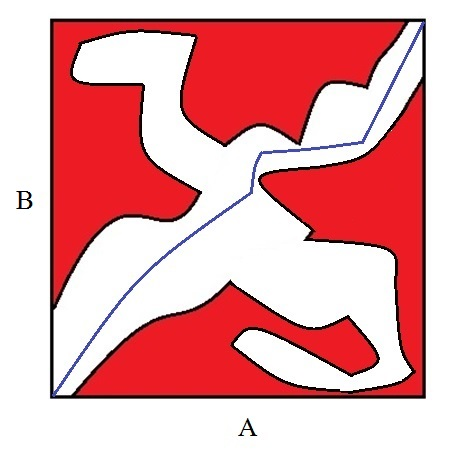
\includegraphics[width=0.75\linewidth]{pics/conf_space2_with_path.jpg}
	\caption{The free space diagram for trajectories $A$ and $B$ and some fixed $\gamma$. The valid regions are in white. The blue monotone path shows one way
to parameterize the curves so the distance between any two matched points is always less than $\gamma$.
}
	\label{fig:conf}
\end{figure}

\vspace{1cm}

In order to find $D_F(u, v)$, one may perform a binary search over the values of
$\gamma$, finding the minimum value for which a valid path exists.
Unfortunately, the free space diagram is defined with conic arcs and thus must support a range of queries on arrangements of conic arcs, which is not easy to implement and costly to use.

The {\it discrete} \Frechet{} distance is a variant in which only discrete
points (or stations) along the trajectories are considered. In this case, the \Frechet{} distance corresponds to a sequence 
of steps done on the two trajectories: in each we advance from a station to its
subsequent point on at least one trajectory. 
The discrete \Frechet{} distance is the maximum distance between any pair of stations considered in this 
parameterization. Note that the discrete \Frechet{} distance gives an upper
bound on the continuous variant and in many cases is relatively close to it.

For a given $\gamma$, we query whether the discrete \Frechet{} distance is
smaller than $\gamma$ as follows. Let $u$ and $v$ be two trajectories. We build a two-dimensional matrix M such that 
$M(i,j) = 1$ if and only if $d(u_i, v_j) < \gamma$, where $d$ is the Euclidean
distance and $u_i, v_j$ are the $i$-th and $j$-th points of $u$ and $v$,
respectively. Next, we test if there is a weakly monotone path of cells with
value 1 from the bottom left of the matrix to its top right, using a
traditional dynamic programming pattern (each step in the path is thus horizontal, vertical
or diagonal for moving on the first trajectory, second trajectory and both
trajectories, respectively).
Such a weakly monotone path corresponds to a parameterization valid for $\gamma$
and thus the existence of such a path is the result of the query.

%With this in mind, we consider a discrete variant of \Frechet{}.
%In our case, we find the discrete version is justified for two main reasons. First, the locations and times in between trajectory points are unknown. A common solution would be to interpolate linearly between points, but clearly it might be just a rough approximation of constant speed between subsequent points. Second, the locations and times themselves are likely to be noisy.
%{\bf SK: do we need to provide so many reasons for using the discrete version? it sounds like we think we shouldn't be doing it, so we are giving many excuses why we do it.}


A simple algorithm for computing the discrete \Frechet{} is to perform 
a binary search over $\gamma$ and find the minimum $\gamma$ valid for the
two trajectories as described above. 
The algorithm takes $O(m^2 \log D_{max})$ time, where $m$ is the link-length of
a trajectory and $D_{max} = \max_{u\in S_1, v\in S_2} D(u, v)$ is the largest distance between any two points in the input.
Note that the above algorithm is not asymptotically optimal; Aggarwal
et al.~\cite{agarwal2012computing} described a more efficient algorithm.

As the discrete version is faster to compute and easier to implement than
the continuous one, we use it in the remainder of
this work.

\subsubsection{Time Associated Setting (TAS)}
\label{sec:tas}
When timestamps are associated with the trajectory samples, trajectories can be
represented as polylines in $\reals^3$ (with $x, y$ and $t$ coordinates).
To compute the distance, we simply sweep the $t = C$ plane for the normalized
parameterizations $t = 0$ to $t = 1$, processing segments intersected simultaneously by the sweeping plane. For each 
such pair, we compute the maximum distance. The maximum value obtained over all
pairs of segments is the similarity measure of the trajectories. It is easy to
verify that the processing time is linear on the trajectory sizes as we traverse both trajectories simultaneously once.

\subsubsection{Partial Time Associated Setting (PTAS)}
\label{sec:ptas}
This case is a generalization of TAS and NTAS. Here a point along an input trajectory may or may not be associated 
with a timestamp. The idea is to solve this variant by modifying the
algorithm for NTAS, restricting the free space diagram with blocking rectangles. Let $T_1$ and $T_2$ be the 
sequences of timestamps of both trajectories sorted by time. Consider two
timestamps $t_1 \in T_1$ and $t_2 \in T_2$ so that $t_1 < t_2$. It follows that
$T_2$ cannot reach $t_2$ before $T_1$ reaches $t_1$.
This constraint defines a {\it forbidden rectangle} in the free space diagram; see Figure~\ref{fig:rects}. 
Given $T_1$ and $T_2$, we process them by increasing timestamps. For each
timestamp visited on one of the trajectories $v$, we take the recent one on the
other trajectory and find the corresponding rectangle. Then we subtract those rectangles from the free space 
diagram to get an instance in which we search for a weakly monotone path. It is
important to observe that each trajectory samples is associated with at most two rectangles that correspond to
constraints with two samples on the other trajectory, appearing before and after
it. Thus, the number of constraining rectangles is linear and does not affect
the complexity of the free space diagram. 
These ideas hold for both the continuous and the discrete versions with the
necessary changes. Detecting the samples inside the forbidden rectangles in the
discrete version can be done in $O(T^3)$ time (recall that $T$ is the trjectory
link length), since one needs to check $O(T^2)$ pairs against $O(T)$ rectangles. However, by using arrangements of segments in $\reals^2$, we can improve the time 
complexity to $O(T^2 \log T)$, relying on the fact that testing the location of a point within the constraining 
rectangles takes $O(\log T)$ time. Based on the characteristics of the forbidden rectangles, they form 
two staircase structures in the free space, touching the bottom-right and the
top-left of the free space respectively; see Fig.~\ref{fig:rects}.

\begin{figure}[htb]
	\centering
	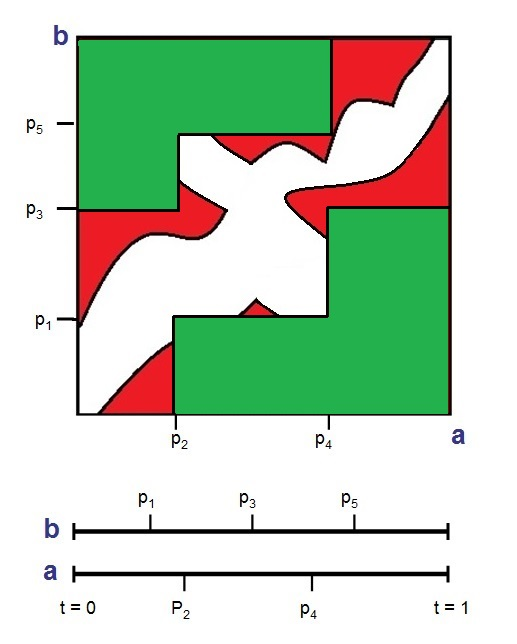
\includegraphics[width=0.98\linewidth]{pics/forb_rect2.jpg}
	\caption{The free space diagram for a pair of trajectories $a$ and $b$ overlayed with forbidden 
	rectangles (in green) that contribute to the invalid parameterization (the red
	areas). The parameterization of the trajectories are depicted below.}
	\label{fig:rects}
\end{figure}

PTAS is practical for cases where the timestamp is given partially. This occurs
when the data is not reliable or when the sensors that report the location/timestamps need
  to save energy and thus report only partial data.
It can also be useful for improving the precision of the distance as we
describe next. Given two trajectories with associated timestamps, instead of
computing the distance as proposed in Section~\ref{sec:tas}, we add sample points in between given sample points. 
If we knew the real timestamps of those new points, we could clearly compute a
possibly more precise \Frechet{} distance with TAS. Nevertheless, by using PTAS,
where only some original points have associated timestamps, we will
find optimal parametric time on the new points, potentially improving the 
precision of the distance. 
This case is even more interesting when we do not model the movement between
samples linearly, but rather with non-linear techniques (e.g., Bazier curves or
high order polynomials). Then we could take points along the approximating
curves to improve the computation.

%%%%%%%%%%%%%%%%%%%%%%%%%%%%%%%%%%%%%%%%%%%%%%%%%%%%%%%%%%%%%%%%%%%%%%%%%%%
%%%%%%%%%%%%%%%%%%%%%%%%%%%%%%%%%%%%%%%%%%%%%%%%%%%%%%%%%%%%%%%%%%%%%%%%%%%
%%%%%%%%%%%%%%%%%%%%%%%%%%%%%%%%%%%%%%%%%%%%%%%%%%%%%%%%%%%%%%%%%%%%%%%%%%%
%%%%%%%%%%%%%%%%%%%%%%%%%%%%%%%%%%%%%%%%%%%%%%%%%%%%%%%%%%%%%%%%%%%%%%%%%%%

% Let $S_1 = \{u^1, \dots, u^n\}$ and $S_1 = \{v^1, \dots, v^n\}$ be two sets of trajectories.
% A straightforward approach (referred to as \emph{brute-force}) for solving the \TMATCH{} problem
% consists of two steps.
% First, we build a complete bipartite graph $G$ with $2n$ vertices corresponding to the trajectories.
% For an edge $(u^i, v^j)$ in $G$, we compute its weight as the distance between the trajectories
% $u^i$ and $v^j$ as discussed in the previous section. The next step is to compute a perfect matching in $G$.
% It is easy to see that the problem of finding a perfect matching minimizing the maximum weight
% can be solved in polynomial time using the classical Hopcroft-Karp algorithm~\cite{matching} or
% by finding a maximum flow in $G$~\cite{din}.
% 
% Let us discuss complexity of the approach. Suppose computing a distance for a pair of trajectories requires
% $R$ steps.
% As discussed earlier, $R = O(T)$ for TAS, $R = O(T^2 \log D_{max})$ for NTAS,
% and $R = O(T^2 \log T)$ for PTAS, where $T$ is the length of trajectories and $D_{max}$ is the largest distance between input trajectories.
% Hence, computing all pairwise distances requires $O(n^2 R)$ time. A standard algorithm for finding a
% perfect matching minimizing the maximum weight uses a binary search on the maximum distance between trajectories, and hence, requires $O(n^{2.5} \log D_{max})$ time.
% Therefore, the total time complexity of the algorithm is $O(n^{2.5} \log D_{max} + n^2 R)$.
% As the length $T$ of trajectories may be large, this is often inefficient in practice.
% Fortunately, in most cases we expect most of the trajectories to be
% far enough (location-wise or time-wise) to be candidates for
% pairing. We next present two approaches to improve the running time of
% the algorithm, depending on the availability of time informatio

\subsection{Locality-Sensitive Hashing}
\label{sec:locality}
\TODO{extend it to other settings}

\paragraph{TAS}
Let us consider the scenario in which timestamps are available. We improve the running time of the
brute-force algorithm by limiting the number of trajectory pairs that can be
potentially matched. On a high level, the idea is based on \emph{locality-sensitive hashing}. For each trajectory
$u \in S_1 \cup S_2$, we compute a hash $h(u)$ so that ``similar'' trajectories (those that can be potentially matched)
get close values. To this end, we consider a trajectory $u$ as a point in $R^T$, and choose a random line in $R^T$ with
origin $p\in R^T$ and direction $q\in R^T$. Given a trajectory $u\in R^T$, let $h(u) \in R$ be so that
$p + h(u)q$ is the projection of $u$ onto the line; that is, the nearest point on the line to $u$.
The projection can be found using the expression $u\cdot (u - q - h(u)u) = 0$, where $\cdot$ denotes a dot product. It is easy to see that such a hash is easy to compute in linear time for each trajectory. Note that
similar trajectories correspond to close points in $R^T$, and therefore, get similar hashes. However, it is also sometimes possible that for the points lying far apart, the computed hashes are close.

Now, instead of considering all pairwise distances,
we fix a constant $k$ and for each trajectory $u\in S_1$, find $k$ trajectories $v\in S_2$ with the closest hashes, that is,
having the smallest values $|h(u) - h(v)|$. It is easy to see that this results in computing $kn \ll n^2$ distances and, hence, a graph $G$ with $kn$ edges. Thus, the complexity of computing pairwise distances is reduced from $O(n^2R)$ to $O(nR)$, and the complexity of finding a matching is reduced from $O(n^{2.5}\log D_{max})$ to $O(n^{1.5}\log D_{max})$.

\paragraph{NTAS}
\begin{enumerate}
\item
Dimensionality  reduction with non-uniform sampling
\vspace{2mm}



\item
Assume $p_{i,j}$ is the  location (vertex) of ant $i$ at time $j$.

\item
Let  the number of time slots be denoted by $M/2$.  That is, a trajectory could be thought of as a point in $\reals^M$.
$$p_{i1}.x, p_{i1}.y, \
p_{i2}.x, p_{i2}.y, \ \dots p_{i,{M\over 2}}.x ,p_{i,{M\over 2}}.y$$
where $p_{i1}.x$ and $p_{i1}.y$ are the $x$ and $y$ coordinates of $p_{i1}$.


\def\vr{{\vec r}}
\def\vmu{{\vec \mu}}

\item
Let $\vr$ denote a random vector in  $R^{M}$. Out goal is to find the projection of each trajectory $\pi$ on the line $\{t\vr| t\in \reals\}$.  That is,
%
$(t\cdot \vr)\cdot (\pi-t\vr)=0$  or in other words $t | \vr|^2= \vr\cdot \pi$, or $t={{ \pi\cdot \vr}\over {|\vr|^2}}$.


\item
We next show how to obtain the value of $t$ in $O(\log M)$ time, when $\pi$ is sampled sparsely.  Let $\vr=(\gamma_1, \gamma_2\dots \gamma_M)$.

%et $e=((p_1, t_1), (p_2, t_2))$

\item
To compute the projection of $\pi'$ on the line $\{t\vr| t\in R\}$. Assume first $\pi$ is a single segment (span from all time)

we need to compute $t$ such that $(t\cdot \vr)\cdot (\pi-t\vr)=0$  or in other words $t | \vr|^2= \vr\cdot \pi$, or $t={{ \pi\cdot \vr}\over {|\vr|^2}}$.

\item
{\bf The case that $\pi$ is a single segment.} ~~
Next assume that $\pi$ consists of a single segment, and  all vertices along $\pi$ are uniformly spread along it, so $p_{ij} = p_{i1}+j\vmu$ where $\vmu= {{   p_{iM}-p_{i1} } \over M} $ and $j=0,1,2\dots M-1$.
Note that $\vmu\in \reals^2$.   Hence if $\vmu=(\mu.x, \mu.y)$, then
$$ \pi\cdot \vr=\mu.x\cdot \sum_{ j =1,3,5\cdots}^{M-1} \gamma_j~~ + ~~
\mu.y  {\sum_{ j =2,4,6 \cdots}^M }  \gamma_j  $$






Pre-computing  $s_{0..M}=\sum_{ j =1,3,5\cdots}^{M-1} \gamma_j $ and $\bar s_{0..M}=  \sum_{ j =1,3,5\cdots}^{M-1} \gamma_j$, we see that  ${ \pi\cdot \vr} $ could be computed in $O(1)$ time.




\end{enumerate}

\section{Matching Algorithm}
\label{sec:alg}

\subsection{Clustering}
\label{sec:clus}

\subsection{Common Route}
\label{sec:common}
We want to combine and compute median trajectories from a set of smaller pieces; see Fig.~\ref{fig:stitch}.

\subsection{Matching using Sequential Bounding Box Balanced Tree}
\label{sec:bottleneck}
\TODO{Need to say something about the two possible matching algorithms we used.}
\TODO{need an experimental evidence that the approach helps.}

In this section we describe how to match the trajectories from both
sets \TODO{Rephrase to clarify what those sets are} based on their similarity.
Formally, we want to find a matching $M = \{m_1, \dots, m_n\}$, where $m_k = (u^i, v^j), 1\le k\le n$ with $u^i \in S_1, v^j \in S_2$ and each trajectory
is matched exactly once. Ideally, a good matching identifies pairs of trajectories that belong to the same entity.
To this end, we are looking for a matching that minimizes the maximum distance between matched trajectories.
Our problem, which we denote by \TMATCH{}, is defined as follows.

\textbf{\TMATCH{}}: Given two sets of trajectories, $S_1 = \{u^1, \dots, u^n\}$ and $S_2 = \{v^1, \dots, v^n\}$, find a matching $M = \{m_1, \dots, m_n\}$, where $m_k = (u^i, v^j)$ with $u^i \in S_1, v^j \in S_2$ that minimizes
$$\max_{i, j} D(u^i, v^j).$$

Matching two sets of trajectories can be viewed as a process of two
steps: computing the pairwise distances of trajectories of different
sets and matching the trajectories based on these distances. If the time taken
to compute the distances is $(O(R(m)))$ where $R(m)$ is the time needed to compute
the distances of trajectories, each of size $\le m$, then the
overall time is $O(n^2 R(m))$. Using the algorithm
by Agarwal ~\cite{agarwal2012computing}, the overall complexity is $O(\frac{n^2 m^2
\log \log m}{\log m})$, which might be unacceptable for large $n$ and $m$.
We observe that in real-world cases, two matching trajectories are
much closer to each other than to many of the other trajectories. Consequently, it seems
desirable to filter out most of the false pairs fast, saving the
time for computing their distances. In the previous section we proposed
the Locality-Sensitive Hashing to efficiently filter out many far pairs.
As there is no guarantee that it will filter out any far pairs, we use another technique
based on a geometric data structure that resembles the well known R-tree 
to filter out far pairs.
We describe this data structure as a part of the complete matching algorithm
and refer to it as \emph{Sequential Bounding Box Balanced Tree} (SBBBT for short). This technique
is applicable for NTAS and PTAS (but not for TAS). Its main usage is to bound each
trajectory in a hierarchical fashion. In the following, we assume that a
bounding box is always axis-aligned.

%\TODO{bottleneck matching, as defined, produces poor results; need to compute 
%a lexicographic bottleneck matching}

\begin{figure}[htb]
	\subfigure[]{
    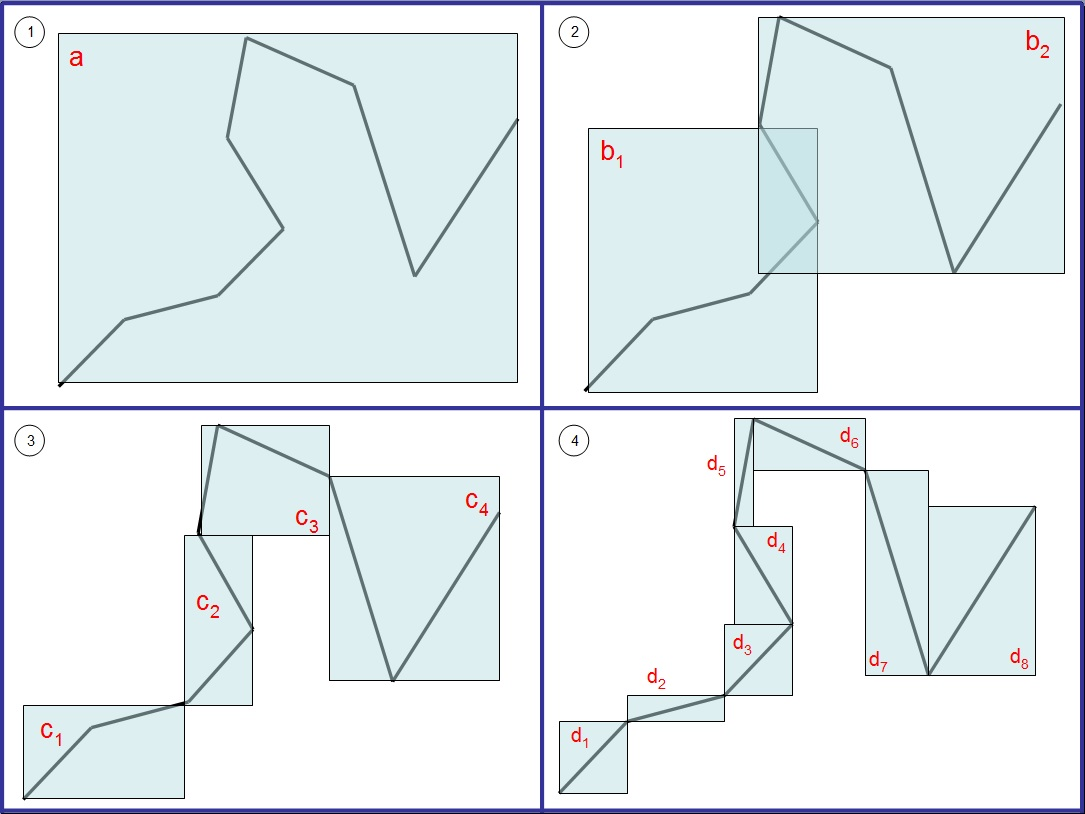
\includegraphics[width=0.48\textwidth]{pics/sbbbt.jpg}}
	\subfigure[]{
    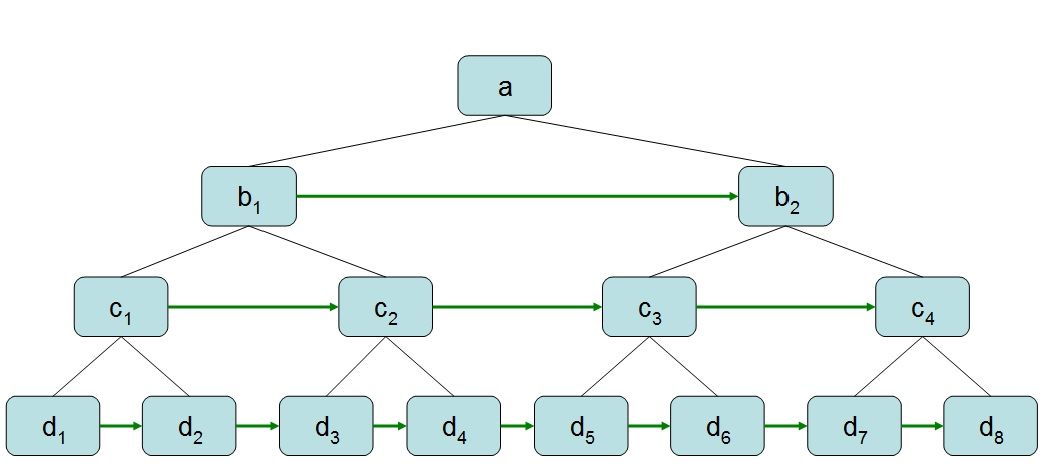
\includegraphics[width=0.48\textwidth]{pics/sbbbt_tree}}
	\caption{(a)~Four levels of bounding boxes of a specific trajectory. (b)~The
	SBBBT of the trajectory. The levels in (b) correspond to
	the boxes in (a) as the symbols indicate.
	Green arrows connect vertices of the same level.}
	\label{fig:sbbbt}
\end{figure}

\begin{definition}
A {\em Sequential Bounding Box Balanced Tree (SBBBT))} is a binary tree
associated with a trajectory and constructed as follows. The root contains the bounding box of the
trajectory. The left and right children of the root correspond to the first and the second part of the trajectory. 
Each child contains the bounding box of the corresponding trajectory part. The rest of the tree is defined 
recursively in the same manner. Each level of the tree (that is an order
of nodes of the same height) contains corresponding pointers to allow its traversal. See Figure ~\ref{fig:sbbbt} for an illustration of SBBBT. 
\end{definition}

Algorithm~\ref{algo:main} is the high level algorithm for computing the
matching. We first construct the SBBBT with $\log m$ levels for every
trajectory. Then we use binary search to find the minimum value of $\gamma$ for which there exists a perfect 
matching with all distances between matched trajectories less than $\gamma$.
We use SBBBT to construct the graph that we inject into the perfect matching
algorithm. It is easy to see that the matching corresponding to the smallest
such $\gamma$ is a bottleneck matching.

\begin{algorithm}[h]
  \caption{Bottleneck Matching}
  \label{algo:main}
  \SetKwInOut{Input}{Input}
  \SetKwInOut{Output}{Output}

  \Input{Trajectories $S_1$ and $S_2$}
  \Output{The optimal bottleneck matching}
  \vspace{1ex}
/* \emph{computing SBBBT} */ \;
  \lForEach{trajectory $u \in S_1 \cup S_2$} {
    create $SBBBT(u)$ \;
  }

  \vspace{1ex}
/* \emph{binary search on $\gamma$} */ \;
  $\gamma_l \leftarrow 0$, $\gamma_r \leftarrow D_{max}$ \;
  \While{$\gamma_l < \gamma_r$} {
    $\gamma \leftarrow (\gamma_l + \gamma_r)/2$ \;
    /* \emph{computing candidate pairs} */ \;
      \ForEach{pair $u \in S_1, v \in S_2$} {
        \lIf{$D_F(SBBBT(u), SBBBT(v)) \le \gamma$}{add $(u, v)$ to $G$}\;
      }
    \vspace{1ex}
    /* \emph{matching} */ \;
    \eIf{a perfect matching with $D_F \le \gamma$ exists in $G$}{$\gamma_l \leftarrow \gamma$}
    {$\gamma_r \leftarrow \gamma$}
  }
\end{algorithm}

Note that the foreach loop in the algorithm is responsible
for determining whether a pair of trajectories is a candidate for a matching and,
if so, it is inserted into $G$. We execute this as follows. Consider a SBBBT tree
constructed for a trajectory $u$. For any level $l \ge 0$, let $SBBBT(u, l)$ be a set of bounding boxes
(rectangles) on level $l$ of the tree. For a pair of trajectories $u\in S_1, v\in S_2$ and for $l \ge 0$, we define the \Frechet{} distance
between $SBBBT(u, l)$ and $SBBBT(v, l)$ in a similar way as the discrete \Frechet{} distance between
trajectories. The difference is that instead of points (the trajectory samples),
we consider rectangles\footnote{In principle this technique will work with any
other shape as well.}.
So instead of jumping from one point to another (on one or two trajectories) we
traverse the rectangles accordingly, generating a sequence of rectangle pairs.
The \Frechet{} distance is now the shortest leash connecting any pair of
rectangles.
Notice that bounding boxes of the tree on some level completely cover the corresponding trajectory.
Hence, if the \Frechet{} distance between $SBBBT(u, l)$ and $SBBBT(v, l)$
for any level $l\ge 0$ exceeds $\gamma$, the \Frechet{} distance between
$u$ and $v$ also exceeds $\gamma$, which is the \Frechet{} distance of the trajectories.
Using this observation, we can check whether $D_F(u, v) \le \gamma$ by
traversing the trees as follows.
If $D_F(SBBBT(u, 0), SBBBT(v, 0)) > \gamma$, then the distance between $u$ and $v$ also exceeds $\gamma$; 
otherwise, proceed with the next level and so on. (See
Figure ~\ref{fig:valid_paths}).
Only if the distance is less than $\gamma$ at all levels, we
compute the \Frechet{} distance of the corresponding trajectories. Note that the
computation cost increases as we descend in the tree. Hence, disqualifying the trajectories early results in significant savings in the 
running time.

To further save time, we store the following information for pairs of
trajectories.
(1)~If the \Frechet{} distance is computed at some iteration, we use this value
instead of recomputing it during subsequent iterations. (2)~If the pair is
filtered out for some $\gamma$ (that is, the \Frechet{} distance is
proven to be greater than $\gamma$), then we do not check it again for larger
values of $\gamma$. Overall, in the worst case, the algorithm for computing a
bottleneck matching has the same complexity as the brute-force algorithm. However, we found significant speedup 
in practice, as discussed in Section~\ref{sec:exper}.


\begin{figure}[htb]
	\centering
	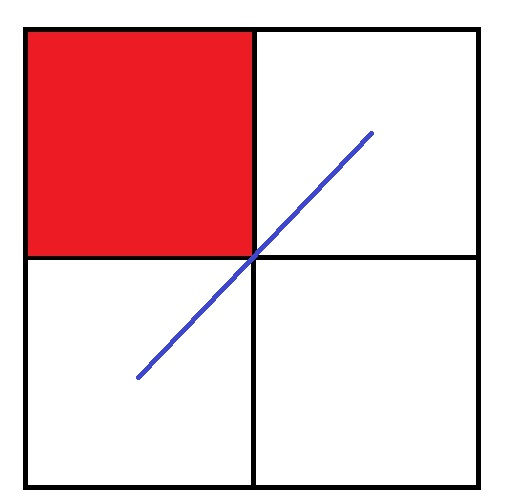
\includegraphics[width=0.49\linewidth]{pics/sq1_with_path.jpg}
	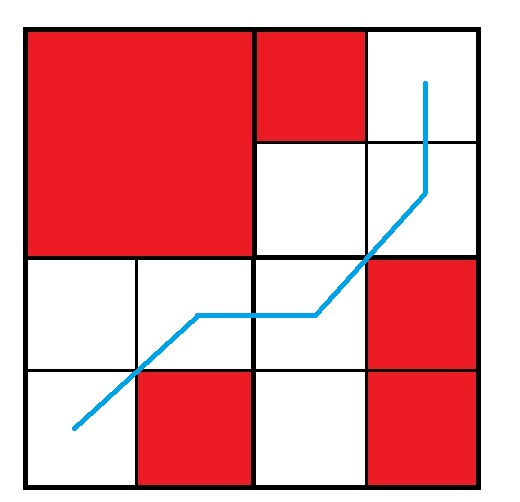
\includegraphics[width=0.49\linewidth]{pics/sq3_with_path.jpg}
	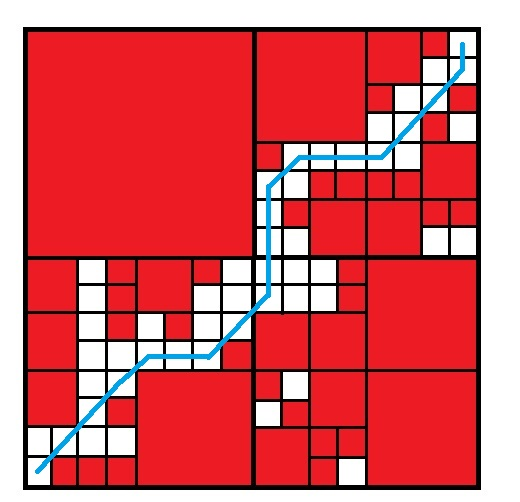
\includegraphics[width=0.49\linewidth]{pics/sq5_with_path.jpg}
	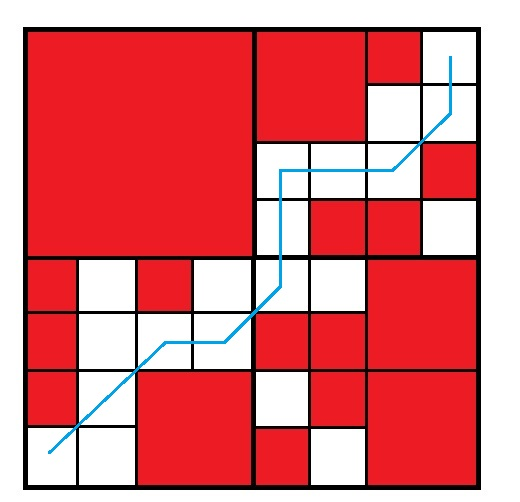
\includegraphics[width=0.49\linewidth]{pics/sq4_with_path.jpg}
	\caption{Computing the \Frechet{} distance with SBBBT.
Decreasing levels (from top-left clockwise) of SBBBT are depicted on the parameterization diagram for a pair of trajectories. Red cells 
represent forbidden parameterization values. In this example, there is a
weakly monotone path from bottom-left to top-right in all levels (in blue). }
	\label{fig:valid_paths}
\end{figure}

% We next describe how we check for the existence of a perfect matching for a
% giving value $\gamma$ in Algorithm~\ref{algo:main}. First, we compute a bipartite graph $G$ with $2n$ vertices in which an edge between 
% two trajectories is present if and only if the trajectories can be potentially matched. To this end, we compute the \Frechet{} distance 
% between $SBBBT(u, l)$ and $SBBBT(v, l)$ for levels $0 \le l \le 3$, and add an edge $(u, v)$ to $G$ if
% the distance is less than $\gamma$. Clearly, this operation can be done efficiently since the number
% of boxes at the levels is relatively small. We expect to filter out most of the pairs of trajectories at this step, and construct a sparse 
% $G$. Second, we check whether there exists a perfect matching in $G$.
% For this purpose, we use the maximum flow algorithm~\cite{din} by adding source and sink vertices to $G$,
% and then iteratively finding augmenting paths in the graph. During the search for an augmenting path,
% we use the corresponding edge $(u, v)$ if the \Frechet{} distance between $u$ and $v$ is less than $\gamma$. Here, we again use the trees 
% $SBBBT(u)$ and $SBBBT(v)$ to speed up the running time. We check up to $\log T$ levels
% of the trees, where $T$ is the length of trajectories. We stress that the actual computation of the \Frechet{} distance
% is performed only if $D_F(SBBBT(u, l), SBBBT(v, l)) \le \gamma$ for all $0 \le l \le \log T$.
% If the maximum flow in $G$ is equal to $n$, then we conclude that there exists a perfect matching for the
% current value $\gamma$.


\begin{figure}[htb]
\centering
    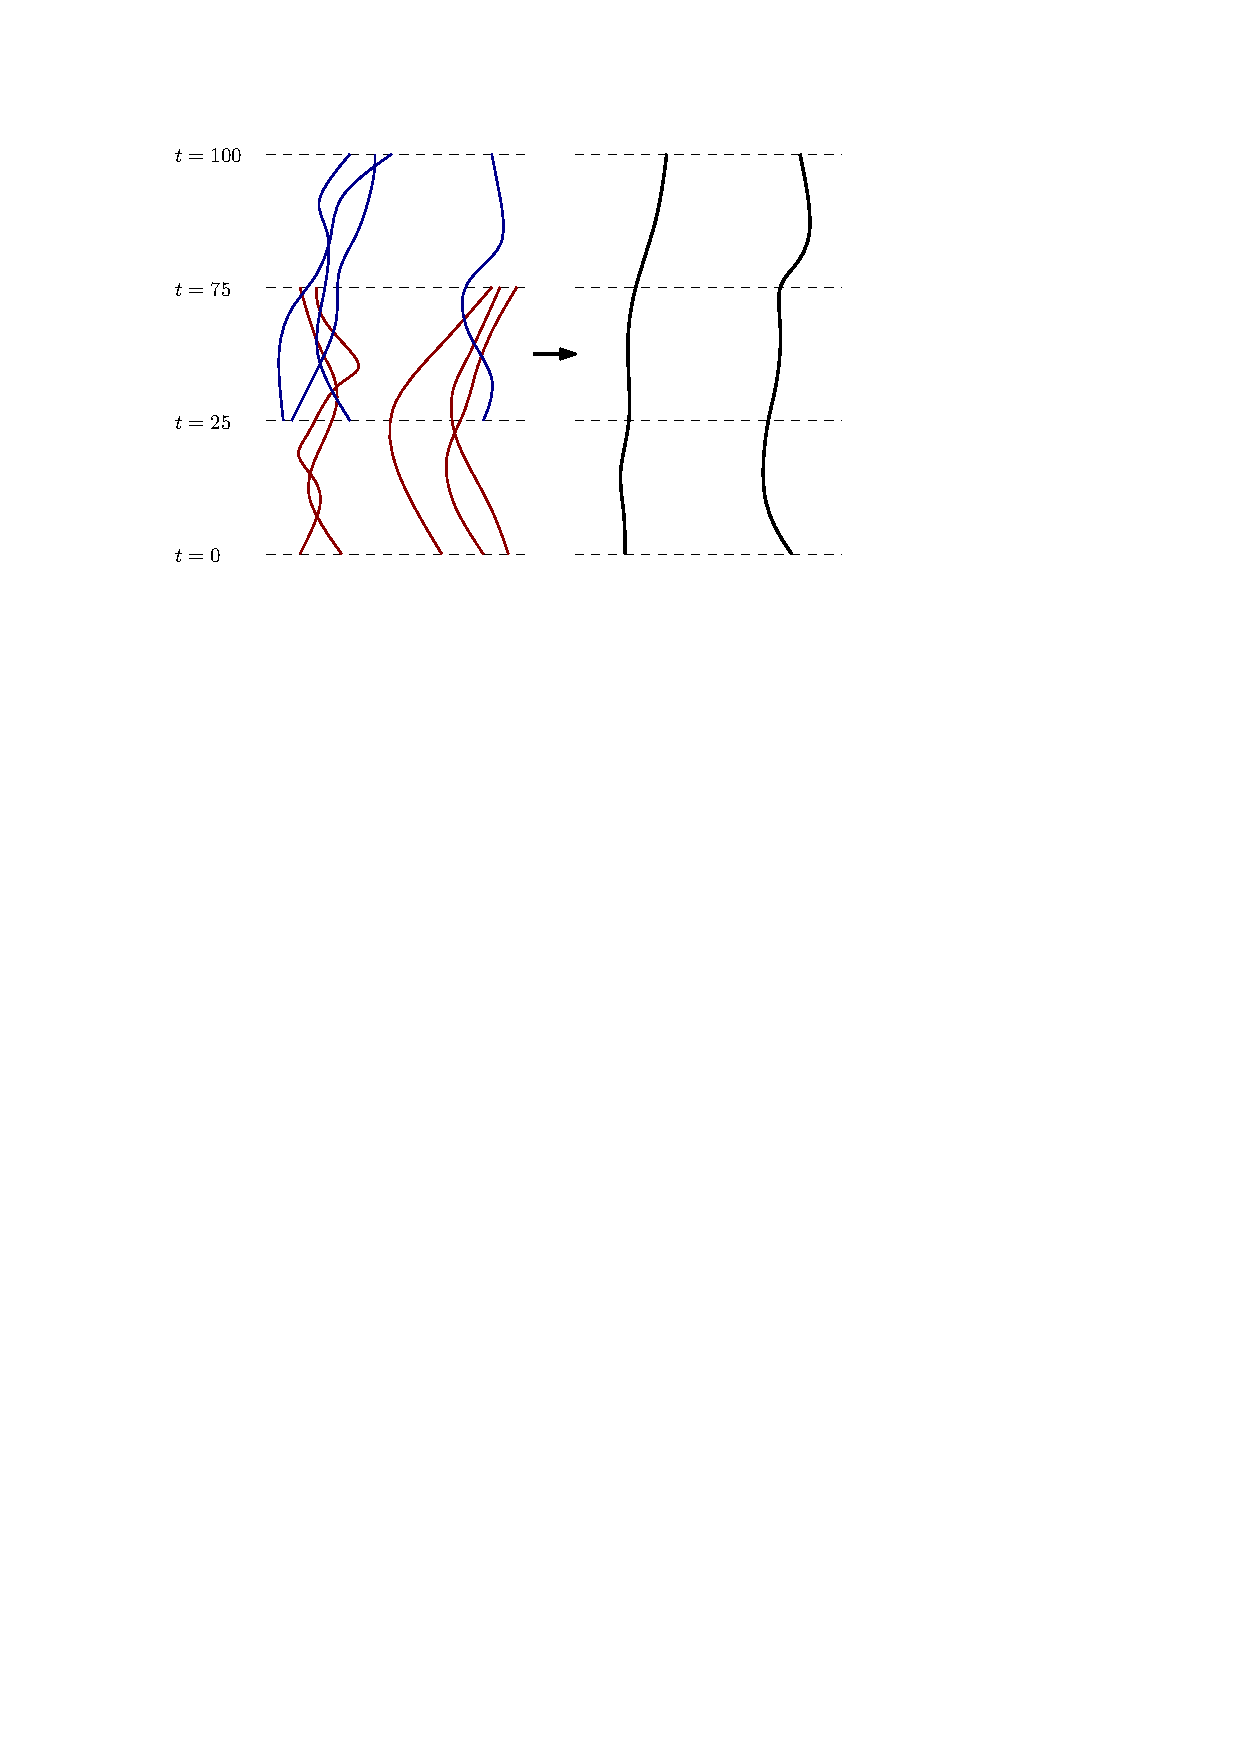
\includegraphics[height=5cm]{pics/stitching}
	\caption{The input (left) is a set of red and blue trajectories. Trajectories of the same color span the same time period. The result (right) is combined black trajectories spanning the entire time period.}
	\label{fig:stitch}
\end{figure}

%%%%%%%%%%%%%%%%%%%%%%%%%%%%%%%%%%%%%%%%%%%%%%%%%%%%%%%%%%%%%%%%%%%%%%%%%%%
%%%%%%%%%%%%%%%%%%%%%%%%%%%%%%%%%%%%%%%%%%%%%%%%%%%%%%%%%%%%%%%%%%%%%%%%%%%
%%%%%%%%%%%%%%%%%%%%%%%%%%%%%%%%%%%%%%%%%%%%%%%%%%%%%%%%%%%%%%%%%%%%%%%%%%%
%%%%%%%%%%%%%%%%%%%%%%%%%%%%%%%%%%%%%%%%%%%%%%%%%%%%%%%%%%%%%%%%%%%%%%%%%%%
\section{Experiments}
\label{sec:exper}
We evaluate our algorithms on four datasets. We start with a real-world collection
of ant trajectories generated by citizen scientists. We then consider two
datasets constructed from route data of vehicle trajectories.
The last one is an artificial dataset that is designed to highlight 
some features and insights about our methods.

\subsection{Citizen Science Trajectories}
\label{sec:ants}
The problem of matching pairs of trajectories naturally arises
in the context of extracting accurate average trajectories of ants
from many (possibly inaccurate) input trajectories contributed by
citizen scientists~\cite{ants}. In this setting, a citizen scientist
plays an online game showing a video of an ant colony; the goal is
to generate a trajectory of a specified ant via mouse clicks.
Citizen scientists track ants during short video segments. In order to
reconstruct a complete ant trajectory, one needs to stitch together
short pieces of overlapping trajectories. Equivalently, given partially
overlapping trajectories, the problem is to identify trajectories
corresponding to the same ant; see Fig.~\ref{fig:ex1}.

\begin{figure}[h!]
    \center
    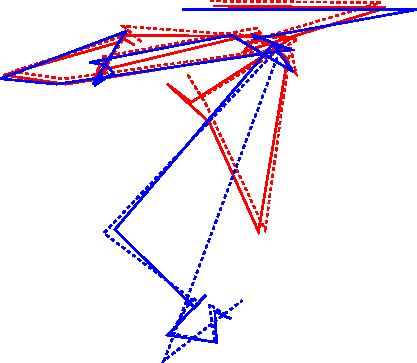
\includegraphics[width=0.25\textwidth]{pics/ant2-6}
    \caption{
4 citizen science trajectories corresponding to two different ants.
Although the trajectories of the blue ant and the red ants are partially overlap,
the matching algorithm is capable to identify 2 pairs of trajectories.}
    \label{fig:ex1}
\end{figure}

To evaluate our algorithms, we work with a video of a {\em
Temnothorax rugatulus} ant colony containing 10,000 frames, recorded
at 30 frames per second. Our dataset consists of 252 citizen-scientist-generated
trajectories for 50 ants, with between 2 and 8 trajectories per ant.
From the data, we construct 150 inputs for our matching algorithm.
Every input consists of 50 pairs of trajectories with different length of overlapping
segments varying from 300 seconds (corresponding to 100 timestamps) to 5 seconds (corresponding to
1 common timestamp). Since the trajectories contain associated time information,
we compute distances as in TA setting and use the matching algorithm described in
Section~\ref{sec:locality}. The bipartite graph $G$ is constructed by applying
locality-sensitive hashing and using $k$ closest trajectories for $k=50$, $k=20$, and $k=10$.
Note that the case with $k=50$ is equivalent to the brute-force algorithm.

\begin{figure}[h!]
    \center
	\subfigure[]{
    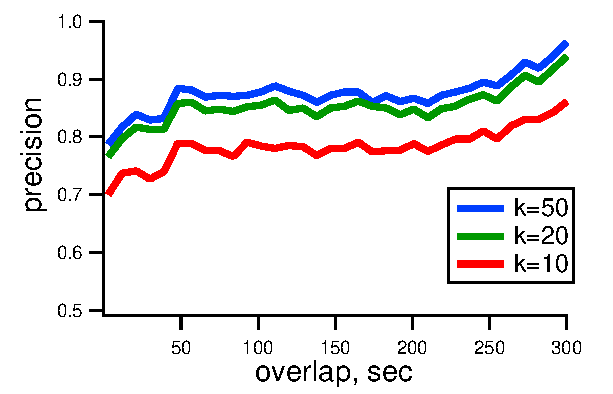
\includegraphics[width=0.34\textwidth]{pics/precision_ants}
    \label{fig:ex3}}
	\subfigure[]{
    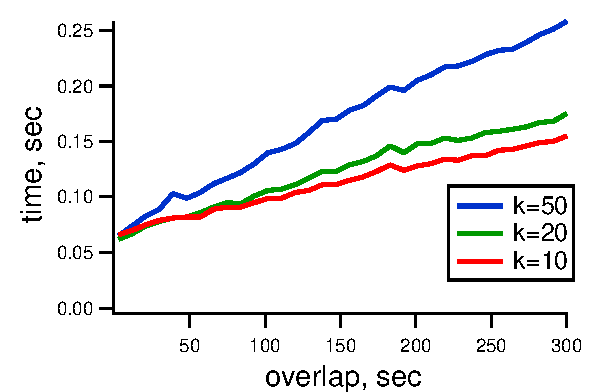
\includegraphics[width=0.34\textwidth]{pics/time_ants}
    \label{fig:ex4}}
\vspace{-0.5cm}
    \caption{The results on the Citizen Science Trajectories dataset. $k$ is the number of ``close'' trajectories used in the locality-sensitive hashing approach.
(a)~Precision ($\frac{\mbox{correctly identified pairs}}{\mbox{all pairs}}$) is higher for trajectories with
longer overlap. (b)~The running time of our algorithm.}
\end{figure}

We compare the results by measuring the precision of the result and the running time
of the algorithm; see Fig.~\ref{fig:ex3} and Fig.~\ref{fig:ex4}.
The \emph{precision} is the percentage of correctly identified pairs
of trajectories, which we know from ground-truth data. As expected, precision is higher for the inputs in which pairs of
trajectories have longer overlap. The brute-force algorithm correctly matches over
$95\%$ pairs of trajectories having 5-minute overlap. As expected, using
locality-sensitive hashing significantly improves the running time,
whie only slightly reducing the accuracy. Specifically, in the setting
where input trajectories have 1-minute overlap and for $k=20$
(which corresponds to $60\%$ fewer considred possible
trajectories) we achive $85\%$ precision (which corresponds to only
$5\%$ reduction in accuracy).

\subsection{Vehicle Trajectories}
We work with two datasets constructed from real-world vehicle trajectories.
The first one contains
public transportation trajectories (busses and trams) on a specific
day in Helsinki. The second one contains ship  trajectories at the
port of Rotterdam; see Fig.~\ref{fig:trajs}. In both cases the trajectories are
represented by geographic coordinates (longitude and latitude), and
no time information is available. The Helsinki dataset contains
4 collections with $20$, $110$, $282$, and $496$ trajectories; the
Rotterdam dataset contains 5 collections with $36$, $52$, $92$, $124$, and $184$
trajectories. The length of trajectories varies from $11$ to $2800$ points with $1400$ on average.
Given a trajectory, we create its {\em paired} trajectory by randomly
moving every point within a disk of radius $r$. We call the radius a
\emph{perturbation} and use $r \in \{0.001, 0.005, 0.01, 0.1\}$ in our
experiments. Note that the value $r=0.01$ corresponds approximately to $10$ kilometers.
Using the data, we constructed $\approx 10^6$ inputs with $40-992$ pairs of
trajectories per input.

\begin{figure}[h!] 	
	\centering
	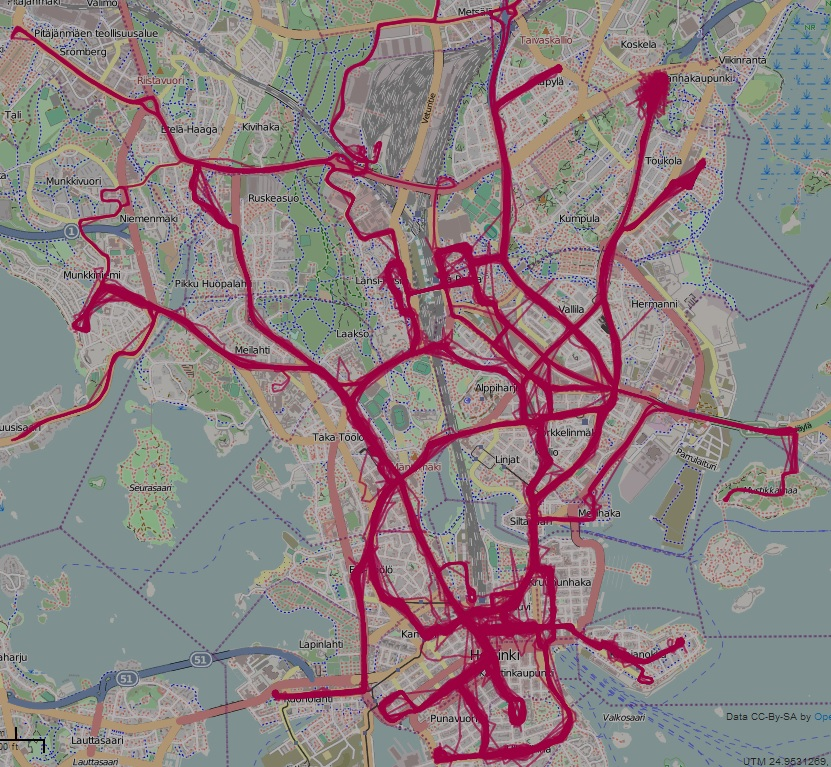
\includegraphics[width=0.75\linewidth]{pics/helTrajs}
~~~
	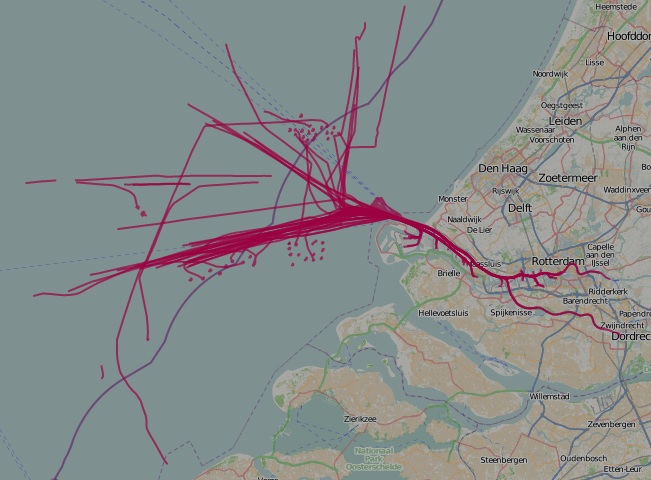
\includegraphics[width=0.75\linewidth]{pics/roterdamTrajs}
	\caption{The trajectories we experimented with: Helsinki public transportation (top) and Ships near and at the port of Rotterdam (bottom).} 	
	\label{fig:trajs}
\end{figure}

The results of our experiments are given in Fig.~\ref{fig:runtime}.
Here we compare the bottleneck matching algorithm
designed for NTA setting computing the discrete \Frechet{} distance
between trajectories. We observe that for the perturbation value $r \le 0.01$
the algorithm correctly identifies all pairs of trajectories, that is, achieves
$100\%$ precision. On the other hand, for $r \ge 1$ none of the algorithms has
a chance to recover correct pairs of trajectories. Hence, in this section we primarily
focus on measuring the running time for smaller values of perturbation.
We compare the basic brute-force algorithm against our new bottleneck
matching algorithm described in Section~\ref{sec:bottleneck}.
We first note that the running time depends on the size of the input; see
Fig.~\ref{fig:runtime}.
The running time also depends on the noise (perturbation value);
larger noise results in longer running time. This can be explained by the
fact that larger noise results in more pairs of trajectories that can be
potentially matched to each other.

\begin{figure}[h!]
	\subfigure[]{
    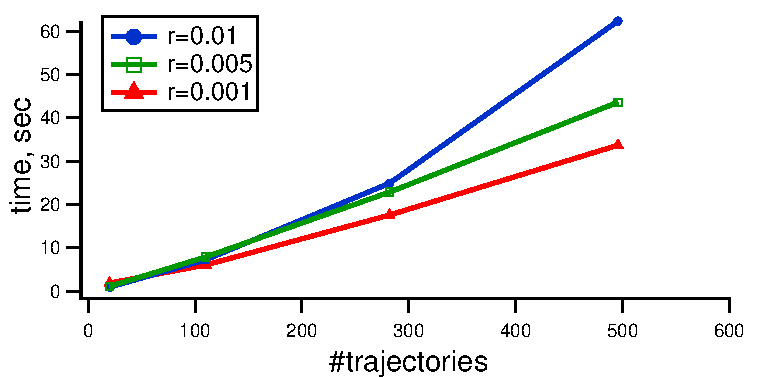
\includegraphics[width=0.42\textwidth]{pics/result_helCompTime_new}}
	\subfigure[]{
    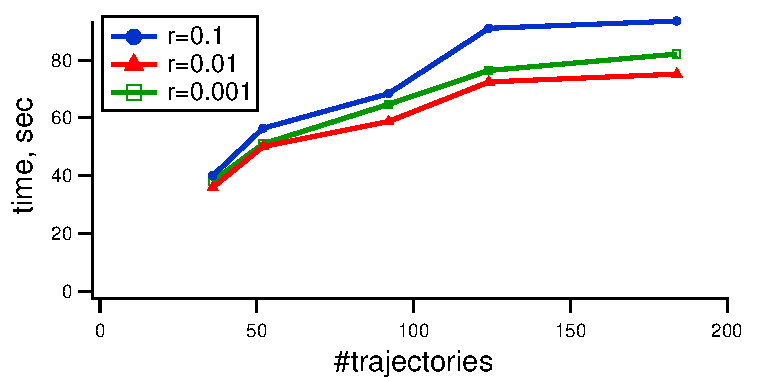
\includegraphics[width=0.42\textwidth]{pics/result_rotCompTime_new}}
	\caption{The running time of the bottleneck matching algorithm on the
(a)~Helsinki and (b)~Rotterdam datasets for different values of perturbation.}
	\label{fig:runtime}
\end{figure}

As the most time-consuming step in the matching algorithms is calculation of
the \Frechet{} distance, we also report on how well our heuristic filters
\Frechet{} computation calls. We define a \emph{saving ratio} as the number
of the pairs of trajectories for which we computed the \Frechet{} distance divided
by the total number of pairs of trajectories. The lower value corresponds
to a better filtering, and the brute-force algorithm has the saving ratio $1$.
The results are presented in Fig.~\ref{fig:ratio}.
We note that for a dataset with $\ge 100$ trajectories, our heuristic using SBBBT
 filters out most of the pairs of trajectories. The actual computation of
the \Frechet{} distance is done only for $\le 2-5\%$ of all pairs. This
corresponds to the $20-50x$ speedup compared to the brute-force algorithm.

\begin{figure}[h!]
	\subfigure[]{
    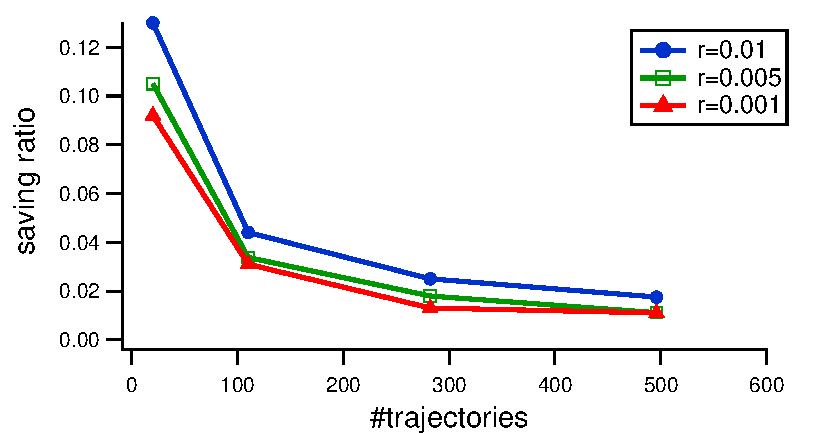
\includegraphics[width=0.42\textwidth]{pics/result_helFretCompRel_new}}
	\subfigure[]{
    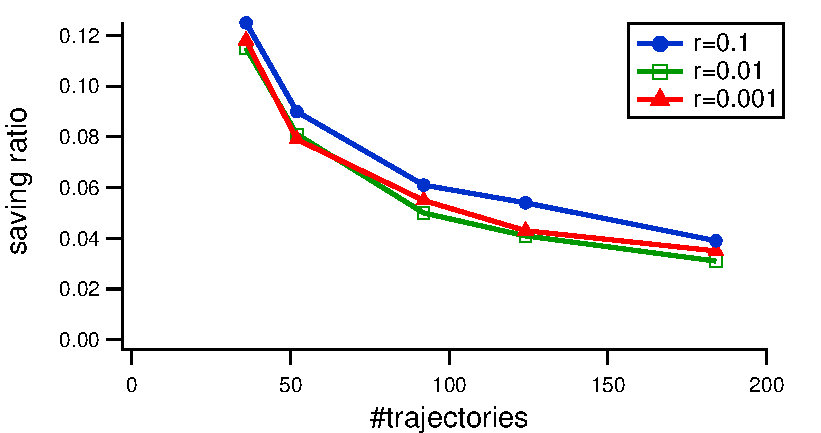
\includegraphics[width=0.4\textwidth]{pics/result_rotFretCompRel_new}}
	\caption{The saving ratio of the bottleneck matching algorithm on the
(a)~Helsinki and (b)~Rotterdam datasets for different values of perturbation.}
	\label{fig:ratio}
\end{figure}


%\begin{figure}[h!]
%	\subfigure[Running time]{
%    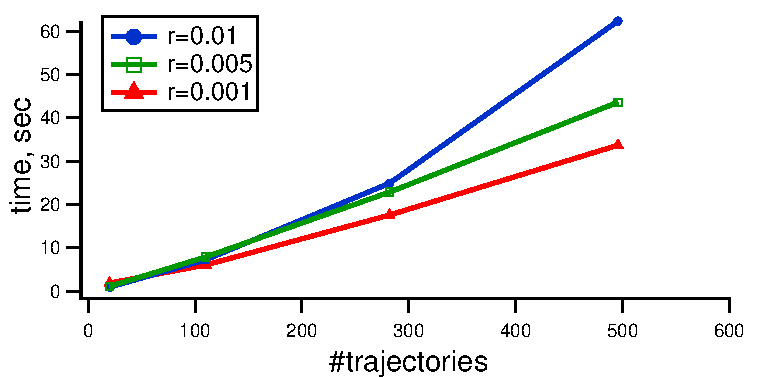
\includegraphics[width=0.42\textwidth]{pics/result_helCompTime_new}}
%	\subfigure[Relative Time vs Brute-Force]{
%    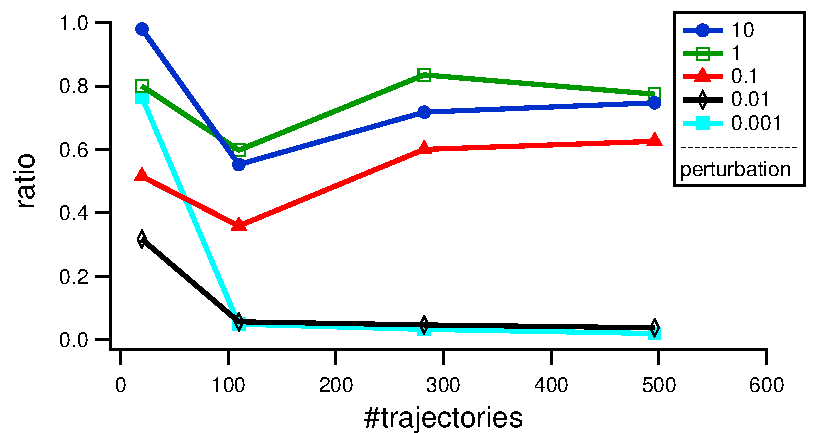
\includegraphics[width=0.42\textwidth]{pics/result_helRelativeTime_new}}
%	\subfigure[\Frechet{} Distance Computation Ratio vs Brute-Force]{
%    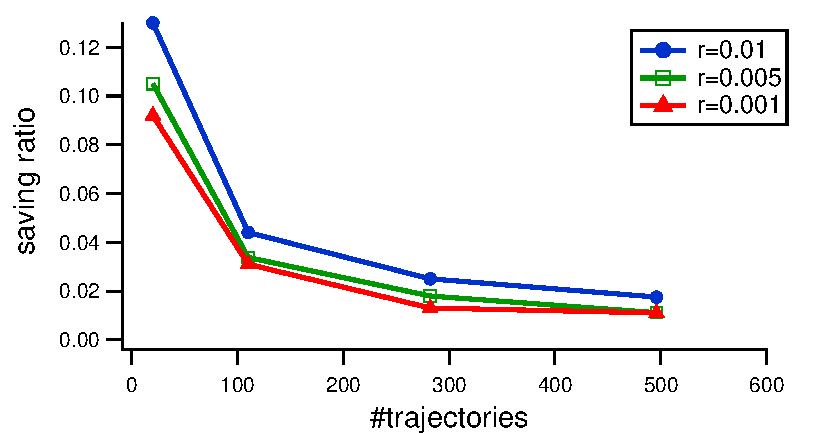
\includegraphics[width=0.42\textwidth]{pics/result_helFretCompRel_new}}
%	\caption{Statistical results obtained for the Helsinki dataset. The left column shows the computation time of running the experiments on different size of input (the number of trajectories and the total sample size characterize the input) and for each different noise magnitude. The middle column compare the results with running the algorithm in a brute-force fashion. It shows the ratio of the running time of both. The right column shows the ratio of the  \Frechet{} distance computation calls to show by how much our algorithm decreased these expensive computation.}
%	\label{fig:real_world_result}
%\end{figure}
%
%\begin{figure}[h!]
%	\subfigure[Relative Time vs Brute-Force]{
%    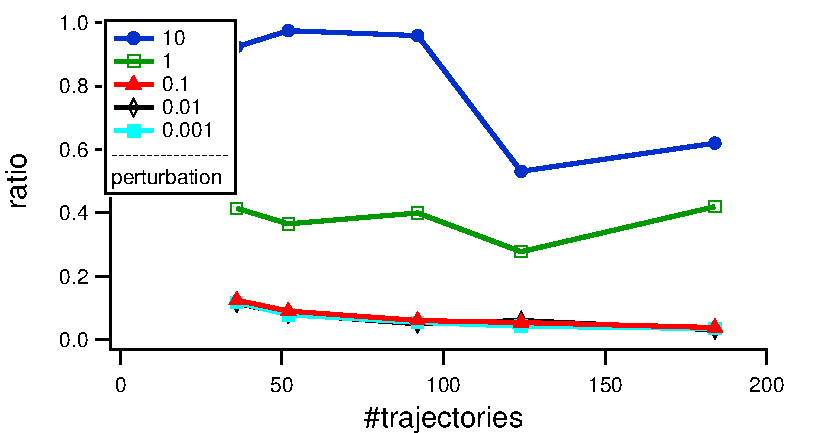
\includegraphics[width=0.4\textwidth]{pics/result_rotRelativeTime_new}}
%	\subfigure[\Frechet{} Distance Computation Ratio vs Brute-Force]{
%    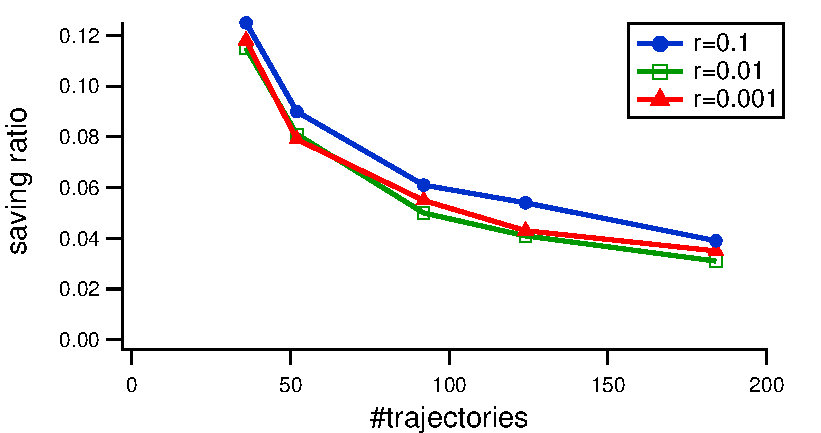
\includegraphics[width=0.4\textwidth]{pics/result_rotFretCompRel_new}}
%	\caption{Results obtained on the Port of Rotterdam dataset.}
%	\label{fig:real_world_result2}
%\end{figure}


\subsection{Artificial Trajectories}
We generated an artificial dataset to further analyze the improvement
of running time and the effect on the quality of the output. The sets $S_1$ and $S_2$ of trajectories
are constructed as follows. Each trajectory $u\in S_1$ is constructed inside a square
of size $10$. Its starting
position and direction $d$ are chosen randomly. Then $u$ grows along $d$ with
steps of unit length until it hits the boundary of the square. When it happens, $d$ is reflected
with slight perturbation to prevent trajectory repetitions. We then generate a
\emph{paired} trajectory $v \in S_2$ by duplicating $u$ and perturbing each
of its points inside a disc centered at the point with radius $r$; see
Fig.~\ref{fig:square}.

%TODO: This way, we create inputs with $200$, $400$, $600$, and $800$ trajectories; see Fig.~\ref{fig:square}.

\begin{figure}[h!] 	
	\centering
	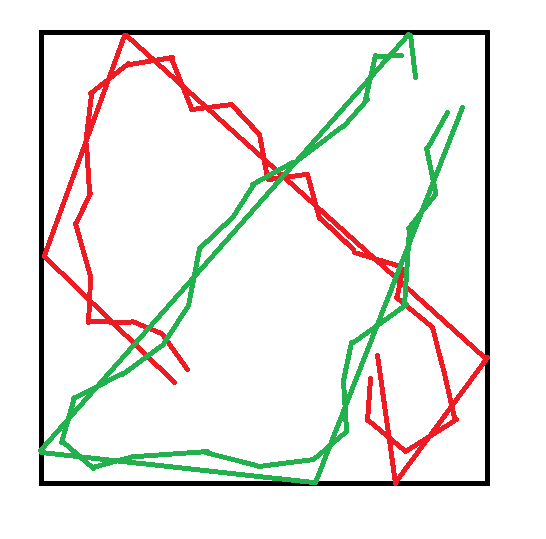
\includegraphics[width=0.6\linewidth]{pics/squareTrajs.png} 	
	\caption{An example of two pairs of generated trajectories inside a square. Each pair is colored with a specific color.} 		 \label{fig:square}
\end{figure}

The motivation of experimenting with this dataset is as follows. Any point along a
trajectory $u \in S_1$ may have many other trajectories close to it at any given timestamp.
However, in the long run, as we move along $u$, we expect that only its paired
trajectory $v$ will be close to $u$. Consider a square of edge length 4.
On average, $25\%$ of the trajectories are close to any point of $u$. On the other hand,
the number of trajectories that are close to it after moving from any point decreases
exponentially. Thus, we expect that non-paired trajectories are filtered
relatively fast using SBBBT. Hence, the \Frechet{}
distance is computed rarely compared to the brute-force algorithm.
With this in mind, we analyze the bottleneck matching algorithm using SBBBT in the NTA
setting.

%\vspace{-0.2cm}
\paragraph{Running Time}
First, we evaluate the running time. In the experiments, we varied the number of
trajectories and the length of a trajectory; see Fig.~\ref{fig:square_stat}.
We use perturbation radius $r=$ for which our algorithm correctly matches all pairs
of trajectories, that is, it has $100\%$ precision. We observed that the number of pairs for which
the algorithm computes the \Frechet{} distance linearly depends on the
input size (the number of trajectories). This explains the linear growth
of the running time in Fig.~\ref{fig:square_stat}.

\begin{figure}[h!]
    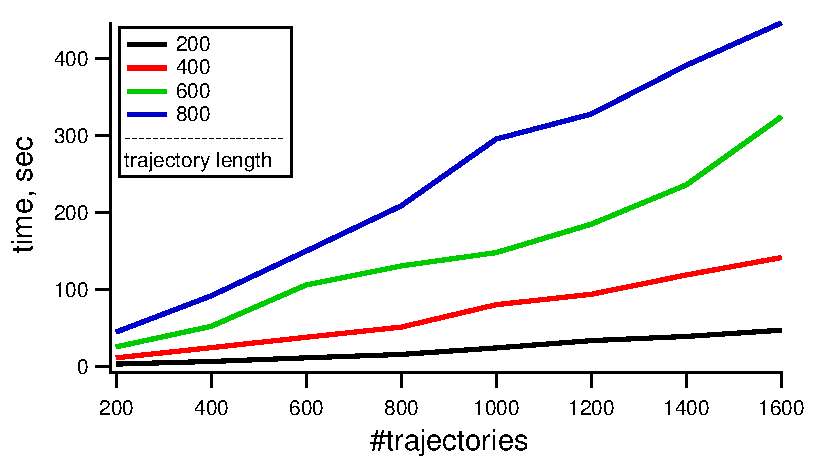
\includegraphics[width=0.42\textwidth]{pics/boxtime1_new}
%	\subfigure[]{
%    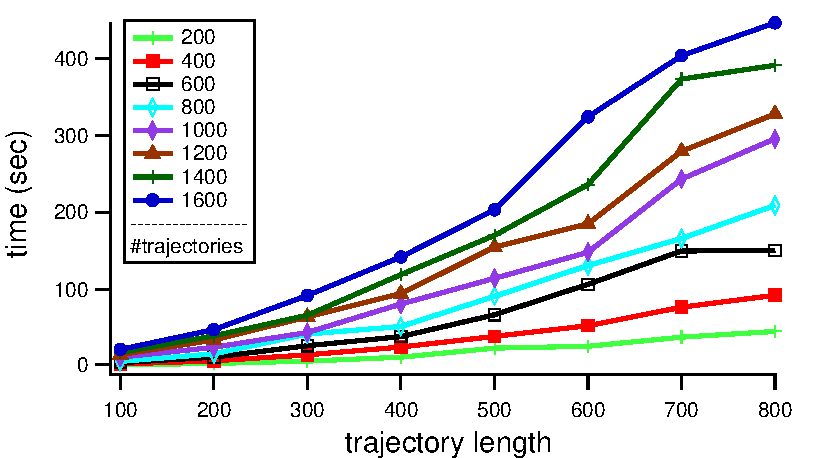
\includegraphics[width=0.48\textwidth]{pics/boxtime2_new}}
	\caption{Results of the Artificial Trajectories experiment. The running time is shown as a function of the number of trajectories for different trajectory lengths.}
	\label{fig:square_stat}
\end{figure}

%\vspace{-0.2cm}
\paragraph{Precision}
In this experiment we set the trajectory length $T=100$, while varying the
input size $n\in \{800, 900, 1000, 1100, 1200\}$ and the perturbation radius $r\in \{1, 2, 3, 5, 6\}$.
We analyze how the perturbation affects precision, that is,
the number of correctly identified pairs divided by
the total number of pairs. The results are shown in Fig.~\ref{fig:preci}.
Not surprisingly, the precision is lower for inputs with larger noise, and
it decreases faster for inputs with more trajectories.
Note, however, that the precision remains steadily over $95\%$ for the entire dataset if $r\le 2$.

 \begin{figure}[h!]
    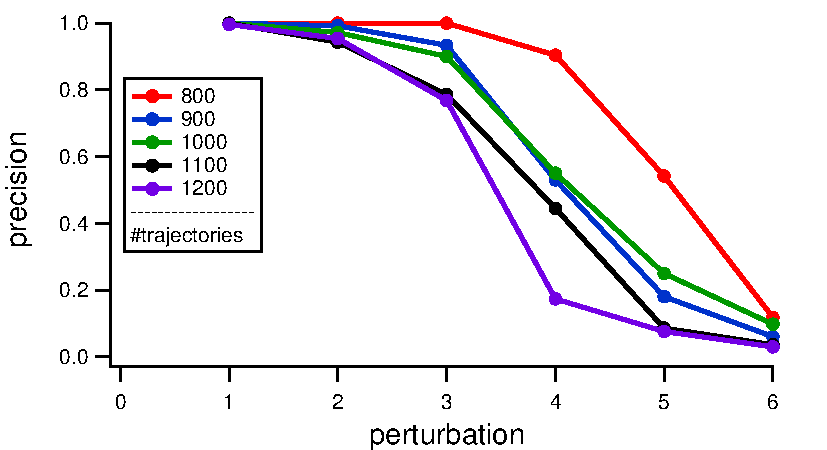
\includegraphics[width=0.48\textwidth]{pics/prec_charts_new}
	\caption{Precision of the results for the Artificial Trajectories dataset.}
	\label{fig:preci}
\end{figure}


%%%%%%%%%%%%%%%%%%%%%%%%%%%%%%%%%%%%%%%%%%%%%%%%%%%%%%%%%%%%%%%%%%%%%%%%%%%
%%%%%%%%%%%%%%%%%%%%%%%%%%%%%%%%%%%%%%%%%%%%%%%%%%%%%%%%%%%%%%%%%%%%%%%%%%%
%%%%%%%%%%%%%%%%%%%%%%%%%%%%%%%%%%%%%%%%%%%%%%%%%%%%%%%%%%%%%%%%%%%%%%%%%%%
%%%%%%%%%%%%%%%%%%%%%%%%%%%%%%%%%%%%%%%%%%%%%%%%%%%%%%%%%%%%%%%%%%%%%%%%%%%
\section{Conclusion and Discussion}
\label{sec:conc}
We presented a novel approach for matching trajectories generated by two independent
resources. We considered three scenarios:
(1)~timestamps are associated with the points of the trajectories, (2)~timestamps are missing, and (3)~some of the points include timestamps.
In every scenario, we presented an efficient algorithm by solving two subproblems.
The first one is to measure similarities of two trajectories, and the second one is to match the trajectories based on the computed similarities.
When timestamps are available, we used locality-sensitive hashing to find a solution with high accuracy.
When no timestamps are known, we measured the similarity using the
\Frechet{} distance. In order to match the trajectories, we use bottleneck
matching (minimizing the maximum distance) and a sequential bounding box balanced tree. To support partial timestamp data, we modified the solution by introducing additional constraints. We demonstrated experimentally that our algorithms yield good results.

An important application of the presented algorithms is tracking ants
(or other insects) in long videos.
For long videos (e.g., hundreds or even thousands of hours), automated tracking methods
are not reliable. Whenever such algorithms loose tracking, the error quickly
accumulates and a trajectory cannot be recovered. Trajectory matching
can be used to resolve this problem. We ask citizen scientists to solve the ``hard ants''
or ``hard trajectory segments'', while tracking
``easy ants'' and/or ``easy trajectory segments''
automatically. Then we apply the matching algorithm for trajectories
and stitch together many short pieces of overlapping trajectories.

A great deal of challenging problems remain. In this work we described
how to match two sets of trajectories. In general, we
may have more than two sets. Already for three sets of trajectories the
problem changes dramatically. First, it is interesting to compute the
\Frechet{} distance in $\reals^3$.
Second, for matching the trajectories we would need to solve a
tripartite matching problem (a matching in hypergraphs in which
vertices contain three elements), which is known to be NP-hard. Also,
our use of augmenting paths will not fit so nicely with more than two
sets. Another direction for future research is to wisely select the
number of levels in the SBBBT. In this paper, we obtained good results
with four levels in the tree. It would be interesting to establish a
good criteria for the determining the number of levels so as to further improve performance.


\bibliographystyle{abbrv}
\bibliography{paper}

\end{document}
